\documentclass[11pt,a4paper]{article}

% ============================================================
%  Redes de Computadoras — OSI vs TCP/IP
%  Apuntes de clase generados a partir de las diapositivas de UNI
%  Documento editable en Overleaf.
% ============================================================

\usepackage[T1]{fontenc}
\usepackage{lmodern}
\usepackage[utf8]{inputenc}
\usepackage[a4paper,margin=2.2cm,top=2.4cm,bottom=2.6cm]{geometry}
\usepackage{xcolor}
\usepackage{tikz}
\usetikzlibrary{arrows.meta,positioning,fit,backgrounds,shapes.multipart,calc}
\usepackage[most]{tcolorbox}
\usepackage{enumitem}
\usepackage{booktabs}
\usepackage{array}
\usepackage{tabularx}
\usepackage{longtable}
\usepackage{titlesec}
\usepackage{fancyhdr}
\usepackage{amsmath}
\usepackage{parskip}
\usepackage{hyperref}

% ---------------- Colores (paleta de los esquemas) ----------------
\definecolor{uniPurple}{HTML}{534AB7}
\definecolor{uniPurpleBg}{HTML}{EEEDFE}
\definecolor{uniTeal}{HTML}{0F6E56}
\definecolor{uniTealBg}{HTML}{E1F5EE}
\definecolor{uniCoral}{HTML}{993C1D}
\definecolor{uniCoralBg}{HTML}{FAECE7}
\definecolor{uniPink}{HTML}{993556}
\definecolor{uniPinkBg}{HTML}{FBEAF0}
\definecolor{uniGray}{HTML}{5F5E5A}
\definecolor{uniGrayBg}{HTML}{F1EFE8}
\definecolor{uniAmber}{HTML}{854F0B}
\definecolor{uniAmberBg}{HTML}{FAEEDA}
\definecolor{uniBlue}{HTML}{185FA5}
\definecolor{uniBlueBg}{HTML}{E6F1FB}
\definecolor{uniDark}{HTML}{0A1E3F}

% ---------------- Títulos de sección ----------------
\titleformat{\section}
  {\normalfont\Large\bfseries\color{uniDark}}
  {\thesection}{0.6em}{}[{\color{uniPurple}\titlerule[1pt]}]
\titleformat{\subsection}
  {\normalfont\large\bfseries\color{uniTeal}}
  {\thesubsection}{0.5em}{}
\titlespacing*{\section}{0pt}{1.6em}{0.8em}
\titlespacing*{\subsection}{0pt}{1.2em}{0.5em}

\pagestyle{fancy}
\fancyhf{}
\fancyhead[L]{\small\textit{Redes de Computadoras --- Modelos OSI y TCP/IP}}
\fancyhead[R]{\small\thepage}
\renewcommand{\headrulewidth}{0.4pt}
\fancyfoot[C]{\small Cristhyan --- UNI, Facultad de Ciencias}

% ---------------- Caja de "dato interesante para el examen" ----------------
\newtcolorbox{examfact}{
  enhanced, breakable,
  colback=uniAmberBg, colframe=uniAmber,
  boxrule=0.6pt, arc=2pt, left=7pt, right=7pt, top=5pt, bottom=5pt,
  fonttitle=\bfseries\small, title={Dato para el examen},
  attach boxed title to top left={yshift=-2mm,xshift=3mm},
  boxed title style={colback=uniAmber, colframe=uniAmber, arc=2pt, boxrule=0pt},
  coltitle=white,
}

\newtcolorbox{analogybox}{
  enhanced, breakable,
  colback=uniTealBg, colframe=uniTeal,
  boxrule=0.6pt, arc=2pt, left=7pt, right=7pt, top=5pt, bottom=5pt,
  fonttitle=\bfseries\small, title={Analogía},
  attach boxed title to top left={yshift=-2mm,xshift=3mm},
  boxed title style={colback=uniTeal, colframe=uniTeal, arc=2pt, boxrule=0pt},
  coltitle=white,
}

\newtcolorbox{defbox}{
  enhanced, breakable,
  colback=uniPurpleBg, colframe=uniPurple,
  boxrule=0.6pt, arc=2pt, left=7pt, right=7pt, top=5pt, bottom=5pt,
  fonttitle=\bfseries\small, title={Definición},
  attach boxed title to top left={yshift=-2mm,xshift=3mm},
  boxed title style={colback=uniPurple, colframe=uniPurple, arc=2pt, boxrule=0pt},
  coltitle=white,
}

% ---------------- Estilo TikZ reutilizable para "cajas de capa" ----------------
\tikzset{
  capa/.style={draw=black!55, thick, rounded corners=3pt, align=center, font=\footnotesize, minimum height=1.05cm, text width=2.6cm, fill=#1},
  capabig/.style={draw=black!55, thick, rounded corners=4pt, align=center, font=\small, minimum height=1.2cm},
  arrflow/.style={-{Latex[length=2.2mm]}, thick},
  contenedor/.style={draw=black!55, thick, rounded corners=8pt, dashed},
}

\title{\vspace{-2cm}\Huge\bfseries\color{uniDark} Modelos de referencia\\[2pt] OSI \textit{vs} TCP/IP}
\author{Apuntes de clase -- Sesion 01 - 04\\ Redes de Computadoras\\ Universidad Nacional de Ingeniería}
\date{}

\begin{document}
\maketitle
\thispagestyle{empty}

\begin{center}
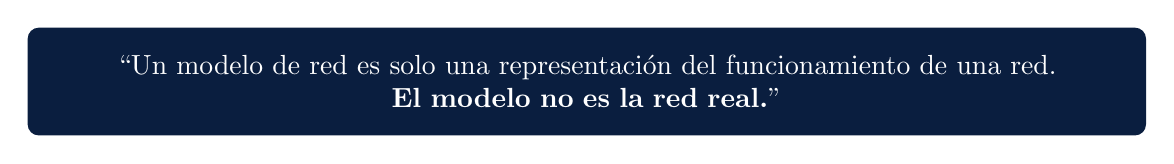
\begin{tikzpicture}
\node[fill=uniDark, text=white, rounded corners=4pt, inner sep=10pt, text width=13.5cm, align=center, font=\normalsize]
  {``Un modelo de red es solo una representación del funcionamiento de una red.\\ \textbf{El modelo no es la red real.}''};
\end{tikzpicture}
\end{center}

\vspace{0.3cm}
\noindent\textbf{Contenido de estos apuntes:} qué es un modelo de referencia, OSI frente a TCP/IP, qué es un protocolo y qué es un estándar, las características de todo protocolo, las 7 capas del modelo OSI una por una (con sus protocolos, su PDU y su encabezado), la tabla maestra Host~Layers/Media~Layers, un ejemplo integrador completo (una videollamada) y el proceso de encapsulamiento de principio a fin.

\newpage
\tableofcontents
\newpage

% ============================================================
\section{¿Qué es un modelo de referencia?}
% ============================================================

\begin{defbox}
Un \textbf{modelo de referencia} es una representación conceptual de cómo dos equipos logran comunicarse, dividiendo ese proceso en capas más pequeñas y manejables. Cada capa tiene una responsabilidad específica y solo se comunica con la capa inmediatamente superior e inferior.
\end{defbox}

OSI y TCP/IP no son ``cosas físicas'' que se puedan tocar: son marcos conceptuales. \textbf{OSI} (\textit{Open Systems Interconnection}) es un modelo \textit{teórico}, creado por la ISO, con \textbf{7 capas}; nació para que cualquier fabricante pudiera diseñar equipos compatibles entre sí. Nunca se implementó tal cual en la práctica, pero se sigue enseñando porque explica el proceso con mucho detalle. \textbf{TCP/IP} es el modelo \textit{práctico}, el que realmente corre Internet hoy; nació del proyecto ARPANET (Departamento de Defensa de EE.\,UU.) y tiene \textbf{4 capas}, porque agrupa varias funciones de OSI en una sola capa.

% ---------------- DIAGRAMA 1: OSI vs TCP/IP ----------------
\begin{figure}[h]
\centering
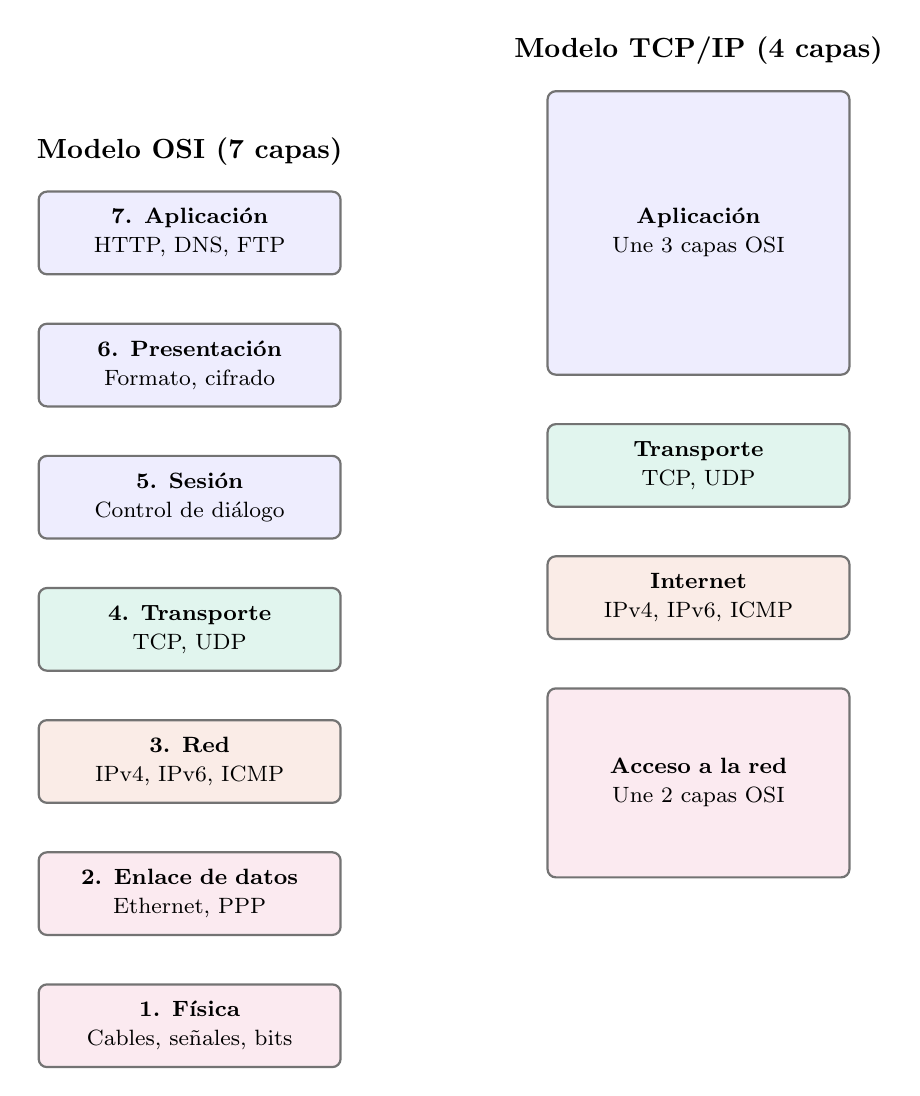
\begin{tikzpicture}[node distance=6mm]
% Columna OSI
\node[capa=uniPurpleBg, text width=3.6cm] (a7) {\textbf{7. Aplicación}\\[1pt]\footnotesize HTTP, DNS, FTP};
\node[capa=uniPurpleBg, text width=3.6cm, below=of a7] (a6) {\textbf{6. Presentación}\\[1pt]\footnotesize Formato, cifrado};
\node[capa=uniPurpleBg, text width=3.6cm, below=of a6] (a5) {\textbf{5. Sesión}\\[1pt]\footnotesize Control de diálogo};
\node[capa=uniTealBg, text width=3.6cm, below=of a5] (a4) {\textbf{4. Transporte}\\[1pt]\footnotesize TCP, UDP};
\node[capa=uniCoralBg, text width=3.6cm, below=of a4] (a3) {\textbf{3. Red}\\[1pt]\footnotesize IPv4, IPv6, ICMP};
\node[capa=uniPinkBg, text width=3.6cm, below=of a3] (a2) {\textbf{2. Enlace de datos}\\[1pt]\footnotesize Ethernet, PPP};
\node[capa=uniPinkBg, text width=3.6cm, below=of a2] (a1) {\textbf{1. Física}\\[1pt]\footnotesize Cables, señales, bits};

\node[above=2mm of a7, font=\bfseries] {Modelo OSI (7 capas)};

% Columna TCP/IP
\node[capa=uniPurpleBg, text width=3.6cm, right=2.6cm of a7, minimum height=3.6cm] (t7) {\textbf{Aplicación}\\[1pt]\footnotesize Une 3 capas OSI};
\node[capa=uniTealBg, text width=3.6cm, below=6mm of t7] (t4) {\textbf{Transporte}\\[1pt]\footnotesize TCP, UDP};
\node[capa=uniCoralBg, text width=3.6cm, below=6mm of t4] (t3) {\textbf{Internet}\\[1pt]\footnotesize IPv4, IPv6, ICMP};
\node[capa=uniPinkBg, text width=3.6cm, below=6mm of t3, minimum height=2.4cm] (t1) {\textbf{Acceso a la red}\\[1pt]\footnotesize Une 2 capas OSI};

\node[above=2mm of t7, font=\bfseries] {Modelo TCP/IP (4 capas)};
\end{tikzpicture}
\caption{Correspondencia entre las 7 capas OSI y las 4 capas TCP/IP. El color agrupa lo que se fusiona.}
\end{figure}

\begin{examfact}
El modelo TCP/IP fusiona Aplicación+Presentación+Sesión de OSI en una sola capa de Aplicación, y Enlace+Física en ``Acceso a la red''. Transporte y Red/Internet quedan igual en ambos modelos (solo Red cambia de nombre a Internet).
\end{examfact}

\subsection*{Diferencias clave}
\begin{center}
\small
\begin{tabularx}{\textwidth}{@{}l X X@{}}
\toprule
\textbf{Aspecto} & \textbf{Modelo OSI} & \textbf{Modelo TCP/IP} \\
\midrule
Creado por & ISO (organización internacional de estandarización) & DoD / proyecto ARPANET \\
N.\textsuperscript{o} de capas & 7 & 4 (a veces 5, separando Enlace y Física) \\
Naturaleza & Teórico / de referencia & Práctico --- el que corre Internet realmente \\
Enfoque & Separa cada función en su propia capa & Agrupa funciones afines en capas generales \\
Uso hoy & Enseñar y diagnosticar por capas & Implementar y diseñar redes reales \\
\bottomrule
\end{tabularx}
\end{center}

\subsection*{El ejemplo general del curso: una carta confidencial}
\begin{analogybox}
El director de una empresa en Lima envía un contrato confidencial al director de una empresa en Tokio. La carta pasa por varios departamentos de su propia empresa antes de salir del edificio (bajando las 7 capas = \textit{encapsulación}), viaja físicamente hasta Japón, y ahí pasa por los mismos departamentos en el orden inverso (subiendo las 7 capas = \textit{desencapsulación}).
\end{analogybox}

\begin{center}
\small
\begin{tabularx}{\textwidth}{@{}l l X l@{}}
\toprule
\textbf{Capa OSI} & \textbf{Rol en la analogía} & \textbf{Qué hace realmente} & \textbf{Protocolos} \\
\midrule
7. Aplicación & El director escribe la carta & Genera el contenido real & HTTP, DNS, FTP \\
6. Presentación & El traductor de la empresa & Traduce, comprime o cifra & TLS/SSL \\
5. Sesión & La secretaria & Abre, coordina y cierra la sesión & NetBIOS, RPC \\
4. Transporte & Logística interna & Divide en partes numeradas, confirma entrega o no & TCP, UDP \\
3. Red & Departamento de rutas & Dirección de destino y mejor camino & IPv4, IPv6, ICMP \\
2. Enlace de datos & El mensajero local & Entrega dentro de la red local (MAC) & Ethernet, PPP \\
1. Física & El camión o avión & Medio de transporte real & Cables, fibra, Wi-Fi \\
\bottomrule
\end{tabularx}
\end{center}

% ---------------- DIAGRAMA 2: PDU por capa ----------------
\begin{figure}[h]
\centering
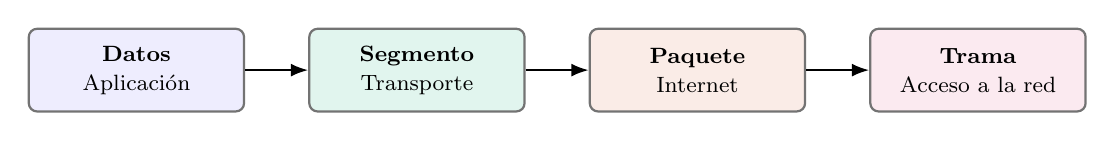
\begin{tikzpicture}[node distance=8mm]
\node[capa=uniPurpleBg, text width=2.5cm] (d) {\textbf{Datos}\\[1pt]\footnotesize Aplicación};
\node[capa=uniTealBg, text width=2.5cm, right=of d] (s) {\textbf{Segmento}\\[1pt]\footnotesize Transporte};
\node[capa=uniCoralBg, text width=2.5cm, right=of s] (p) {\textbf{Paquete}\\[1pt]\footnotesize Internet};
\node[capa=uniPinkBg, text width=2.5cm, right=of p] (f) {\textbf{Trama}\\[1pt]\footnotesize Acceso a la red};
\draw[arrflow] (d) -- (s);
\draw[arrflow] (s) -- (p);
\draw[arrflow] (p) -- (f);
\end{tikzpicture}
\caption{Nombre de la unidad de datos (PDU) en cada capa. Después de ``Trama'' ya no hay más envoltorio: se convierte en bits.}
\end{figure}

\newpage
% ============================================================
\section{¿Qué es un protocolo de red?}
% ============================================================

\begin{defbox}
Un \textbf{protocolo de red} es un conjunto de reglas que dos dispositivos deben aceptar y seguir para que la comunicación funcione correctamente.
\end{defbox}

\begin{analogybox}
Una vendedora y un cliente que no hablan el mismo idioma necesitan comunicarse. Antes de poder intercambiar el pedido deben resolver tres preguntas: (1) ¿qué método de comunicación usar? --- prueban señas, no funciona, acuerdan usar notas escritas; (2) ¿qué idioma usar? --- prueban japonés y español, terminan acordando inglés; (3) ¿deben confirmar que el mensaje llegó bien? --- el cliente pide ``tres camisas negras, talla mediana'', la vendedora repite el pedido, el cliente confirma. La comunicación solo funciona porque \textbf{ambos aceptaron las mismas reglas antes de empezar}, sin negociarlas cada vez porque ya están definidas de antemano en el estándar (HTTP, TCP, Ethernet, etc.).
\end{analogybox}

\begin{center}
\small
\begin{tabularx}{\textwidth}{@{}X X@{}}
\toprule
\textbf{En la tienda (analogía)} & \textbf{En una red (protocolo real)} \\
\midrule
Método de comunicación: señas $\to$ notas escritas & Medio y protocolo: Wi-Fi, Ethernet, HTTP\ldots \\
Idioma común: acuerdan hablar inglés & Codificación del mensaje: mismo formato de datos \\
Confirmar recepción: repite el pedido & Acuse de recibo (ACK): TCP confirma; UDP no \\
\bottomrule
\end{tabularx}
\end{center}

\subsection*{Los cinco elementos que define todo protocolo}
\begin{itemize}[leftmargin=1.4em, itemsep=2pt]
\item \textbf{Codificación del mensaje} --- cómo se convierte la idea en algo transmisible.
\item \textbf{Formato y encapsulamiento} --- cómo se estructura para que el receptor sepa dónde empieza y termina cada parte.
\item \textbf{Tamaño del mensaje} --- si es muy largo, hay que dividirlo en partes más pequeñas.
\item \textbf{Temporización (timing)} --- a qué velocidad se envía y en qué orden se espera la respuesta.
\item \textbf{Opciones de entrega} --- a una sola persona, a varias, o a todas (unicast, multicast, broadcast), y si necesita confirmación.
\end{itemize}

\newpage
% ============================================================
\section{Estándar de red \textit{versus} protocolo de red}
% ============================================================

\begin{analogybox}
Un \textbf{estándar} es como el reglamento de construcción de carreteras: ancho de carriles, tipo de asfalto, señalización --- para que cualquier fabricante de autos pueda circular ahí (interoperabilidad). Un \textbf{protocolo} es como las reglas de tránsito que los conductores siguen ya sobre esa carretera: quién tiene el paso en un cruce, cuándo detenerse. Reglas puntuales para una interacción específica, no para construir toda la infraestructura.
\end{analogybox}

\begin{center}
\small
\begin{tabularx}{\textwidth}{@{}l X X@{}}
\toprule
\textbf{Característica} & \textbf{Estándar de red} & \textbf{Protocolo de red} \\
\midrule
Definición & Especificaciones técnicas de cómo deben implementarse dispositivos o tecnologías & Reglas y procedimientos que rigen la comunicación de datos \\
Propósito & Garantizar interoperabilidad y compatibilidad entre fabricantes & Definir cómo se formatean, transmiten, reciben y procesan los datos \\
Naturaleza & Documento técnico con especificaciones & Reglas implementadas en software o hardware \\
Alcance & Amplio: desde capa física hasta capa de aplicación & Puntual: una función o tarea específica \\
Ejemplos & IEEE 802.3 (Ethernet), IEEE 802.11 (Wi-Fi), modelo OSI & TCP, IP, HTTP \\
Relación & Los protocolos se implementan de acuerdo con los estándares & Los protocolos siguen los estándares para garantizar interoperabilidad \\
\bottomrule
\end{tabularx}
\end{center}

% ---------------- DIAGRAMA 4: estándar contiene protocolo ----------------
\begin{figure}[h]
\centering
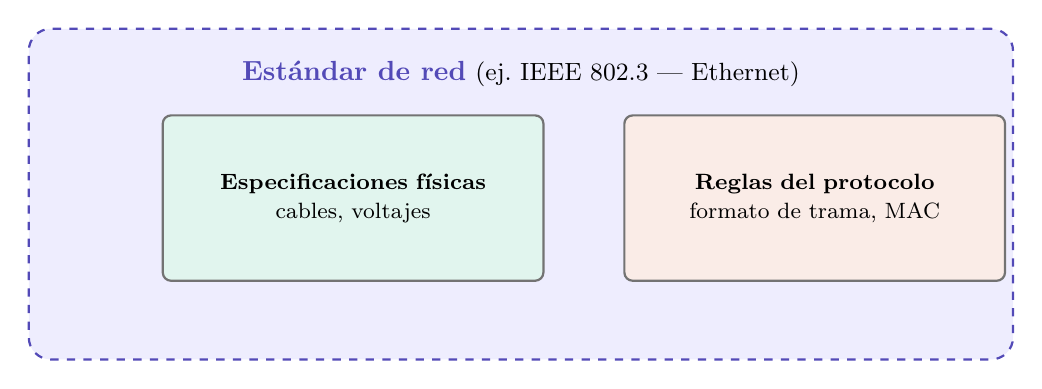
\begin{tikzpicture}
\node[contenedor, draw=uniPurple, fill=uniPurpleBg, minimum width=12.5cm, minimum height=4.2cm] (outer) {};
\node[anchor=north, yshift=-3mm] at (outer.north) {\textbf{\color{uniPurple} Estándar de red} \small(ej.\ IEEE~802.3 --- Ethernet)};

\node[capa=uniTealBg, text width=4.6cm, minimum height=2.1cm, below left=1.1cm and -0.3cm of outer.north] (fis) {\textbf{Especificaciones físicas}\\[1pt]\footnotesize cables, voltajes};
\node[capa=uniCoralBg, text width=4.6cm, minimum height=2.1cm, right=1cm of fis] (prot) {\textbf{Reglas del protocolo}\\[1pt]\footnotesize formato de trama, MAC};
\end{tikzpicture}
\caption{El protocolo vive \emph{adentro} del estándar, nunca al revés.}
\end{figure}

\begin{examfact}
El modelo OSI es, en el fondo, un estándar/modelo de referencia (dice cómo debería organizarse todo); HTTP, TCP o IP son protocolos concretos que operan dentro de esa organización.
\end{examfact}

\newpage
% ============================================================
\section{Características de un protocolo}
% ============================================================

\begin{center}
\small
\begin{tabularx}{\textwidth}{@{}l X X@{}}
\toprule
\textbf{Característica} & \textbf{Descripción} & \textbf{Ejemplo} \\
\midrule
Formato & Estructura, orden y tipo de los datos transmitidos & Encabezado IP, encabezado TCP \\
Tamaño del mensaje & Tamaño máximo de los datos que se pueden transmitir en un PDU & MTU de Ethernet: 1500 bytes; MSS de TCP \\
Sincronización & Coordina velocidad de transmisión y recepción entre dispositivos & NTP (entre dispositivos); números de secuencia de TCP (entre emisor y receptor) \\
Codificación & Cómo se convierten los datos a un formato transmisible & ASCII (7 bits); UTF-8 (1--4 bytes, incluye ASCII) \\
Encapsulamiento & Agregar encabezado y ``cola'' a los datos al bajar por las capas & PDU-Ethernet-\{PDU-IP-[PDU-TCP]\} \\
Patrón del mensaje & Secuencia y formato de los mensajes para establecer, mantener y finalizar una comunicación & Saludo de tres vías de TCP; solicitud-respuesta de HTTP \\
\bottomrule
\end{tabularx}
\end{center}

\subsection*{Tamaño del mensaje: la relación MSS--MTU}
\[
\textbf{MSS} = \textbf{MTU} - 40\ \text{bytes} \qquad (20\ \text{bytes IP} + 20\ \text{bytes TCP})
\]
Con Ethernet estándar (MTU~=~1500~bytes), el MSS típico es \textbf{1460 bytes} para los datos reales de la aplicación. Si un paquete excede el MTU, la capa de Red debe fragmentarlo.

\subsection*{Sincronización: dos mecanismos, no confundirlos}
\textbf{NTP} sincroniza el reloj de \emph{todos} los dispositivos de una red entre sí (corre sobre UDP, puerto 123). Los \textbf{números de secuencia de TCP} no sincronizan relojes: sincronizan el \emph{ritmo} de envío/recepción entre solo dos extremos.

\subsection*{Encapsulamiento: encabezado \emph{y} cola}
\begin{examfact}
La capa de \textbf{Enlace de datos} es la única que agrega encabezado \textbf{y} cola (el FCS, \textit{Frame Check Sequence}), usada para detectar errores de transmisión mediante CRC. Ninguna otra capa agrega algo al final del mensaje, solo al principio.
\end{examfact}

\subsection*{Patrón del mensaje: el saludo de tres vías de TCP}
% ---------------- DIAGRAMA 5: three-way handshake ----------------
\begin{figure}[h]
\centering
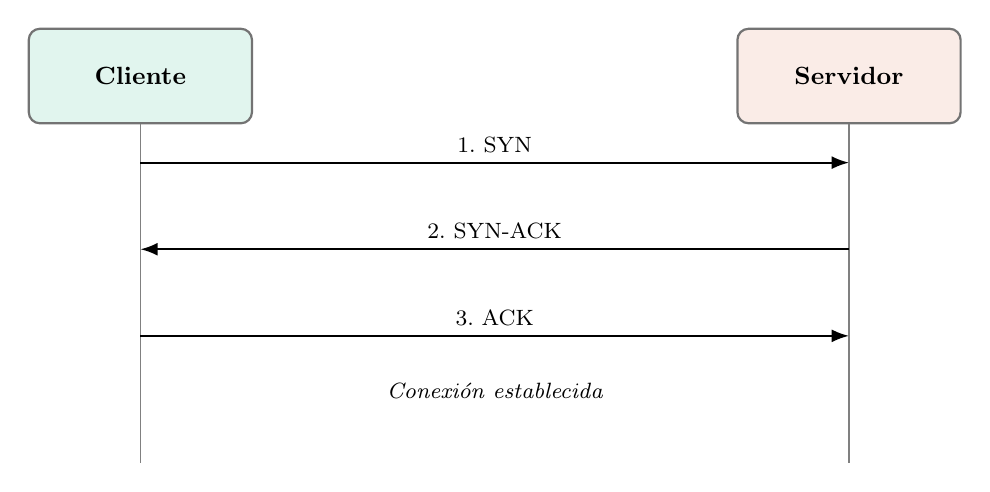
\begin{tikzpicture}[node distance=0mm]
\node[capabig, fill=uniTealBg, text width=2.6cm] (cli) at (0,5) {\textbf{Cliente}};
\node[capabig, fill=uniCoralBg, text width=2.6cm] (srv) at (9,5) {\textbf{Servidor}};
\draw[black!50] (cli.south) -- ++(0,-4.3);
\draw[black!50] (srv.south) -- ++(0,-4.3);

\draw[arrflow] (0,3.9) -- node[above, font=\footnotesize]{1.\ SYN} (9,3.9);
\draw[arrflow] (9,2.8) -- node[above, font=\footnotesize]{2.\ SYN-ACK} (0,2.8);
\draw[arrflow] (0,1.7) -- node[above, font=\footnotesize]{3.\ ACK} (9,1.7);
\node[font=\footnotesize\itshape] at (4.5,1.0) {Conexión establecida};
\end{tikzpicture}
\caption{El SYN no solo ``toca la puerta'': lleva un número de secuencia inicial. El SYN-ACK confirma ese número y manda el suyo propio. El ACK final confirma el del servidor.}
\end{figure}

\begin{examfact}
El three-way handshake no solo abre la conexión: intercambia y confirma números de secuencia iniciales en ambas direcciones, base para que TCP pueda detectar pérdida o desorden de datos después.
\end{examfact}

\subsection*{Resumen de datos clave de esta sección}
\begin{itemize}[leftmargin=1.4em, itemsep=2pt]
\item MSS = MTU $-$ 40 bytes. Con MTU 1500 (Ethernet), MSS típico = 1460 bytes.
\item Solo Enlace de datos agrega encabezado \emph{y} cola (FCS/CRC).
\item UTF-8 es retrocompatible con ASCII byte por byte en sus primeros 128 caracteres.
\item TCP es orientado a conexión (necesita handshake); UDP no lo es --- por eso NTP (sobre UDP) sincroniza relojes sin ``conectar'' antes.
\item HTTP es \textit{stateless}: cada petición se resuelve de forma independiente, salvo que se usen cookies o sesiones.
\item La fragmentación (por MTU) la hace la capa de \textbf{Red}, no Transporte ni Enlace.
\end{itemize}

\newpage
% ============================================================
\section{Capa 7 --- Aplicación}
% ============================================================
\textit{Da a las aplicaciones acceso a los recursos o servicios de la red.}

\begin{examfact}
La capa de aplicación \textbf{no es la aplicación en sí} (no es el navegador ni el cliente de correo). Es el conjunto de protocolos que esa aplicación usa para acceder a servicios de red.
\end{examfact}

% ---------------- DIAGRAMA 6: protocolos capa aplicación ----------------
\begin{figure}[h]
\centering
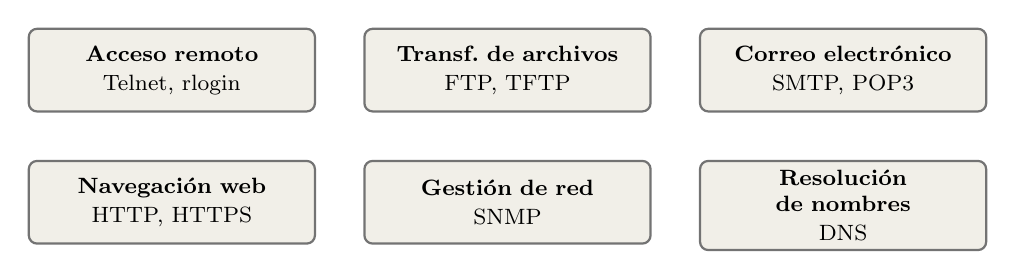
\begin{tikzpicture}[node distance=6mm and 6mm]
\node[capa=uniGrayBg, text width=3.4cm] (a) {\textbf{Acceso remoto}\\[1pt]\footnotesize Telnet, rlogin};
\node[capa=uniGrayBg, text width=3.4cm, right=of a] (b) {\textbf{Transf.\ de archivos}\\[1pt]\footnotesize FTP, TFTP};
\node[capa=uniGrayBg, text width=3.4cm, right=of b] (c) {\textbf{Correo electrónico}\\[1pt]\footnotesize SMTP, POP3};
\node[capa=uniGrayBg, text width=3.4cm, below=of a] (d) {\textbf{Navegación web}\\[1pt]\footnotesize HTTP, HTTPS};
\node[capa=uniGrayBg, text width=3.4cm, below=of b] (e) {\textbf{Gestión de red}\\[1pt]\footnotesize SNMP};
\node[capa=uniGrayBg, text width=3.4cm, below=of c] (f) {\textbf{Resolución de nombres}\\[1pt]\footnotesize DNS};
\end{tikzpicture}
\caption{Protocolos de capa 7 agrupados por función.}
\end{figure}

\textbf{FTP vs.\ TFTP:} FTP corre sobre TCP, usa autenticación y dos canales (control y datos). TFTP corre sobre UDP, sin autenticación, mucho más simple --- se usa para cargar firmware al arrancar un equipo. \textbf{Telnet} manda todo en texto plano, incluida la contraseña; por eso fue reemplazado por SSH en el uso real (aunque SSH no aparezca en listas de libros más antiguos).

\subsection*{PDU: ``L7 Data''}
Cuando el usuario genera datos, la capa de Aplicación los empaqueta como \textbf{L7 Data} y los entrega hacia abajo, a la capa de Presentación. En el sentido contrario, recibe el L7 Data que subió desde las capas inferiores y se lo entrega al usuario.

\begin{examfact}
X.500, FTAM y X.400 (que a veces aparecen en diagramas de esta capa) son protocolos \emph{puros de OSI} que casi nadie usa hoy: X.500 = servicio de directorio, FTAM = equivalente OSI de FTP, X.400 = mensajería OSI. El mundo real usa DNS, FTP y SMTP en su lugar.
\end{examfact}

\subsection*{Puertos que suelen preguntar}
\begin{center}
\small
\begin{tabular}{@{}llllll@{}}
\toprule
HTTP & HTTPS & FTP & SMTP & POP3 & DNS \\
80 & 443 & 20/21 & 25 & 110 & 53 \\
\midrule
Telnet & SNMP & & & & \\
23 & 161/162 & & & & \\
\bottomrule
\end{tabular}
\end{center}

\newpage
% ============================================================
\section{Capa 5 --- Sesión}
% ============================================================
\textit{Asegura el establecimiento y la terminación de la sesión.}

Protocolos: \textbf{RPC} (ejecuta procedimientos en un sistema remoto desde uno local), \textbf{SCP} (Session Control Protocol, de DECnet Phase IV --- no confundir con el ``Secure Copy'' de SSH), \textbf{NetBIOS} (servicios de sesión en LAN), \textbf{SIP} (inicia/termina llamadas VoIP), \textbf{H.323} (estándar UIT para videoconferencia, competidor de SIP) y \textbf{AppleTalk} (su componente de sesión, ASP).

% ---------------- DIAGRAMA: syn TCP vs syn sesión ----------------
\begin{figure}[h]
\centering
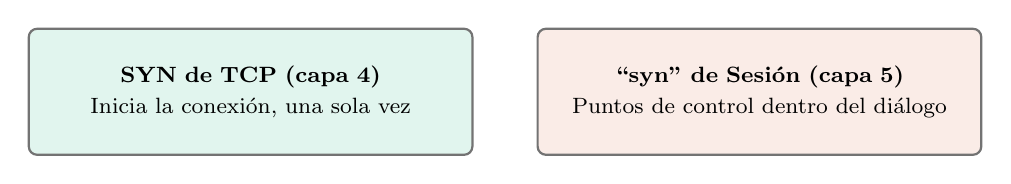
\begin{tikzpicture}[node distance=8mm]
\node[capa=uniTealBg, text width=5.4cm, minimum height=1.6cm] (t) {\textbf{SYN de TCP (capa 4)}\\[2pt]\footnotesize Inicia la conexión, una sola vez};
\node[capa=uniCoralBg, text width=5.4cm, minimum height=1.6cm, right=of t] (s) {\textbf{``syn'' de Sesión (capa 5)}\\[2pt]\footnotesize Puntos de control dentro del diálogo};
\end{tikzpicture}
\caption{No confundir: el SYN de TCP ocurre una vez al abrir la conexión; los puntos de sincronización de la capa de Sesión son \emph{checkpoints repetidos} a lo largo de un diálogo largo.}
\end{figure}

Los puntos de sincronización de la capa de Sesión funcionan como puntos de guardado en un videojuego: si se corta la conexión, no se vuelve al principio, se vuelve al último ``syn''. En el diagrama de encapsulamiento, esos puntos dividen el bloque de datos en segmentos, y todo va envuelto con el encabezado \textbf{H5} antes de bajar como ``L5 Data'' hacia Transporte.

\begin{examfact}
TCP/IP no tiene capa de sesión propia: sus funciones quedan fusionadas en la única capa de Aplicación de TCP/IP. Por eso casi nunca se escucha hablar de ``protocolos de sesión'' fuera del contexto académico de OSI.
\end{examfact}

\begin{examfact}
La capa de Sesión soporta \textit{full-duplex} (ambos hablan a la vez) y \textit{half-duplex} (se turnan).
\end{examfact}

\newpage
% ============================================================
\section{Capa 6 --- Presentación}
% ============================================================
\textit{Responsable de traducir, cifrar y comprimir los datos.}

Formatos y protocolos: Rich Text Format, MIDI, QuickTime, MPEG, JPEG, TLS (SSL), DOCX, XLSX, XML.

\begin{examfact}
DOCX y XLSX son, literalmente, archivos \textbf{ZIP que contienen XML adentro}. Cambiar la extensión a \texttt{.zip} y abrirlo muestra una carpeta con archivos \texttt{.xml} --- así guardan Word y Excel el formato desde 2007.
\end{examfact}

\begin{examfact}
\textbf{MIDI no guarda sonido real}, a diferencia de un MP3 o WAV: guarda instrucciones (``toca esta nota, con este instrumento, a este volumen, en este momento'') --- más parecido a una partitura que a una grabación.
\end{examfact}

TCP/IP no tiene capa de presentación propia (sus funciones se fusionan en la capa de Aplicación); por eso TLS a veces se describe como parte de la capa de aplicación, y otras como una ``capa de transporte segura'' encima de TCP, según el libro.

% ---------------- DIAGRAMA 8: orden de procesamiento ----------------
\begin{figure}[h]
\centering
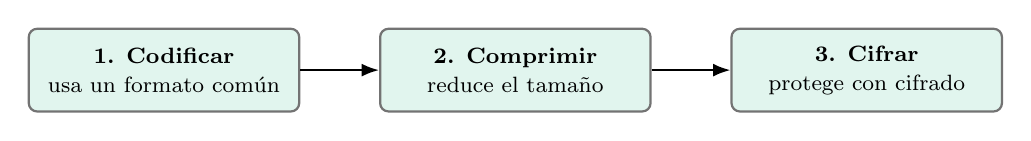
\begin{tikzpicture}[node distance=10mm]
\node[capa=uniTealBg, text width=3.2cm] (c1) {\textbf{1. Codificar}\\[1pt]\footnotesize usa un formato común};
\node[capa=uniTealBg, text width=3.2cm, right=of c1] (c2) {\textbf{2. Comprimir}\\[1pt]\footnotesize reduce el tamaño};
\node[capa=uniTealBg, text width=3.2cm, right=of c2] (c3) {\textbf{3. Cifrar}\\[1pt]\footnotesize protege con cifrado};
\draw[arrflow] (c1) -- (c2);
\draw[arrflow] (c2) -- (c3);
\end{tikzpicture}
\caption{Orden correcto de procesamiento en la capa de Presentación.}
\end{figure}

\begin{examfact}
El orden importa: los datos cifrados se ven como ruido aleatorio (eso es justamente lo que hace bueno a un cifrado), y un compresor funciona buscando patrones repetidos. Si ya no hay patrones porque el cifrado los destruyó, comprimir después de cifrar no ahorra casi nada de espacio. Por eso siempre se comprime primero y se cifra al final.
\end{examfact}

Al igual que en la capa de Sesión, aquí se agrega un encabezado propio (\textbf{H6}) antes de pasar los datos hacia abajo como ``L6 Data''.

\newpage
% ============================================================
\section{Capa 4 --- Transporte}
% ============================================================
\textit{Permite el transporte de datos de la máquina origen a la de destino.} PDU: \textbf{Segmento (TCP)} / \textbf{Datagrama (UDP)}.

\begin{examfact}
La capa de \textbf{Red} (IP) lleva el paquete a la \textbf{máquina} correcta; la capa de \textbf{Transporte} lo lleva al \textbf{proceso o aplicación} correcta \emph{dentro} de esa máquina, usando números de puerto.
\end{examfact}

% ---------------- DIAGRAMA 9: entrega por puerto ----------------
\begin{figure}[h]
\centering
\resizebox{0.92\textwidth}{!}{%
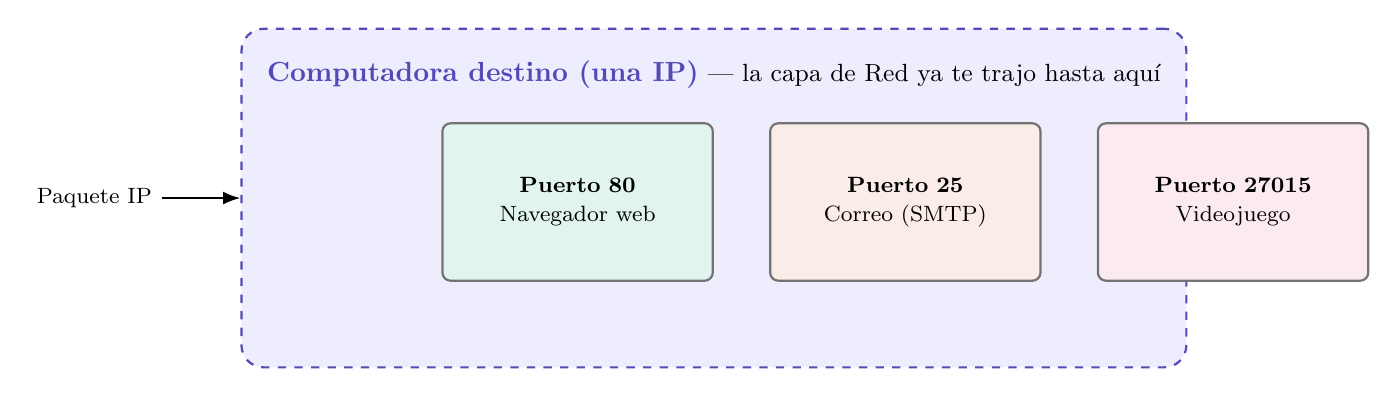
\begin{tikzpicture}
\node[contenedor, draw=uniPurple, fill=uniPurpleBg, minimum width=12cm, minimum height=4.3cm] (outer) {};
\node[anchor=north, yshift=-3mm] at (outer.north) {\textbf{\color{uniPurple}Computadora destino (una IP)} \small--- la capa de Red ya te trajo hasta aquí};

\node[capa=uniTealBg, text width=3.2cm, minimum height=2.0cm, below left=1.2cm and 0cm of outer.north] (p1) {\textbf{Puerto 80}\\[1pt]\footnotesize Navegador web};
\node[capa=uniCoralBg, text width=3.2cm, minimum height=2.0cm, right=7mm of p1] (p2) {\textbf{Puerto 25}\\[1pt]\footnotesize Correo (SMTP)};
\node[capa=uniPinkBg, text width=3.2cm, minimum height=2.0cm, right=7mm of p2] (p3) {\textbf{Puerto 27015}\\[1pt]\footnotesize Videojuego};

\node[left=1.0cm of outer, font=\footnotesize] (ext) {Paquete IP};
\draw[arrflow] (ext) -- (outer.west);
\end{tikzpicture}%
}
\caption{La IP te lleva a la casa correcta (la computadora); el puerto te lleva a la habitación correcta (el proceso).}
\end{figure}

\subsection*{Segmentación: el diagrama de encapsulamiento}
Cuando llega un bloque grande de datos desde la capa de Sesión (L5 Data), la capa de Transporte no lo manda entero: lo \textbf{divide en varios segmentos más pequeños} (limitados por el MSS), le agrega su encabezado \textbf{H4} a cada uno (puerto origen/destino y número de secuencia), y los baja de forma independiente a la capa de Red. En el receptor, los segmentos se reordenan usando los números de secuencia y se reensamblan en el bloque original.

\begin{examfact}
No confundir \textbf{segmentación} (capa 4, según el MSS) con \textbf{fragmentación} (capa 3, forzada por el MTU del medio físico). Son dos procesos de ``partir en pedazos'' en capas distintas, con causas distintas.
\end{examfact}

\subsection*{TCP \textit{versus} UDP}
\begin{center}
\small
\begin{tabularx}{\textwidth}{@{}l X X@{}}
\toprule
\textbf{Característica} & \textbf{TCP} & \textbf{UDP} \\
\midrule
Orientación a conexión & Sí --- requiere handshake & No --- envía directo \\
Confiabilidad & Garantiza entrega; retransmite lo perdido & No garantiza nada \\
Control de flujo/congestión & Sí, con ventana deslizante & No \\
Orden de entrega & Garantizado (números de secuencia) & No garantizado \\
Tamaño de encabezado & 20 bytes mínimo & 8 bytes \\
Velocidad / overhead & Más lento, más overhead & Más rápido, mínimo overhead \\
Casos de uso & HTTP, FTP, SMTP & DNS, streaming, VoIP, juegos, NTP \\
\bottomrule
\end{tabularx}
\end{center}

\begin{examfact}
Dato moderno: HTTP/3 en realidad corre sobre UDP, no TCP; reimplementa la confiabilidad en la propia aplicación (protocolo QUIC) para evitar ciertos retrasos que TCP introduce.
\end{examfact}

\newpage
% ============================================================
\section{Capa 3 --- Red}
% ============================================================
\textit{Provee \textit{internetworking} y movimiento de paquetes.} PDU: \textbf{Paquete}.

Protocolos: \textbf{IP} (direccionamiento lógico y ruteo, \textit{best-effort}: no garantiza entrega ni orden), \textbf{IPsec} (cifra/autentica paquetes IP completos, base de la mayoría de VPN), \textbf{ICMP} (diagnóstico y control --- \texttt{ping}, \texttt{traceroute}; no usa puertos ni TCP/UDP, va directo sobre IP), \textbf{MPLS} (etiquetas cortas para acelerar el reenvío en redes de operador), \textbf{ARP} (IP~$\to$~MAC dentro de la red local) y \textbf{RARP} (MAC~$\to$~IP, hoy obsoleto, reemplazado por DHCP).

% ---------------- DIAGRAMA 10: zona 2.5 ----------------
\begin{figure}[h]
\centering
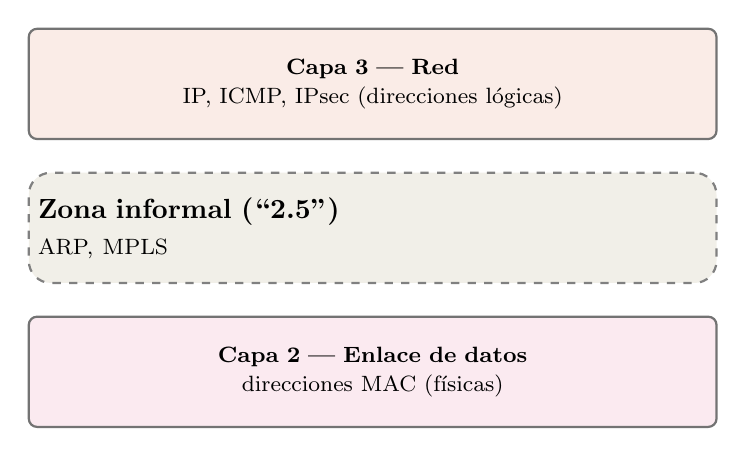
\begin{tikzpicture}[node distance=4mm]
\node[capa=uniCoralBg, text width=8.5cm, minimum height=1.4cm] (l3) {\textbf{Capa 3 --- Red}\\[1pt]\footnotesize IP, ICMP, IPsec (direcciones lógicas)};
\node[contenedor, draw=black!50, fill=uniGrayBg, text width=8.5cm, minimum height=1.4cm, below=of l3] (l25) {\textbf{Zona informal (``2.5'')}\\[1pt]\footnotesize ARP, MPLS};
\node[capa=uniPinkBg, text width=8.5cm, minimum height=1.4cm, below=of l25] (l2) {\textbf{Capa 2 --- Enlace de datos}\\[1pt]\footnotesize direcciones MAC (físicas)};
\end{tikzpicture}
\caption{ARP y MPLS ocupan la frontera entre capa 3 y capa 2 --- por eso muchos libros hablan informalmente de ``capa 2.5''.}
\end{figure}

\begin{examfact}
ARP usa direcciones IP (capa 3) para producir una dirección MAC (capa 2), y su mensaje va directo dentro de una trama de Enlace de datos, sin encabezado IP propio. Es el ejemplo clásico de protocolo que no encaja limpio en una sola capa.
\end{examfact}

\begin{examfact}
IPsec y TLS ambos cifran, pero en capas distintas: IPsec protege el paquete IP completo (nivel de red); TLS protege una conexión de aplicación específica (nivel de presentación/aplicación).
\end{examfact}

El diagrama de encapsulamiento sigue el mismo patrón: L4~Data baja desde Transporte, la capa de Red agrega su encabezado \textbf{H3}, y el conjunto pasa a llamarse oficialmente \textbf{Paquete} antes de bajar como L3~Data hacia Enlace de datos.

\newpage
% ============================================================
\section{Capa 2 --- Enlace de datos}
% ============================================================
\textit{Organiza los bits en tramas.} PDU: \textbf{Trama}.

% ---------------- DIAGRAMA 11: categorías capa enlace ----------------
\begin{figure}[h]
\centering
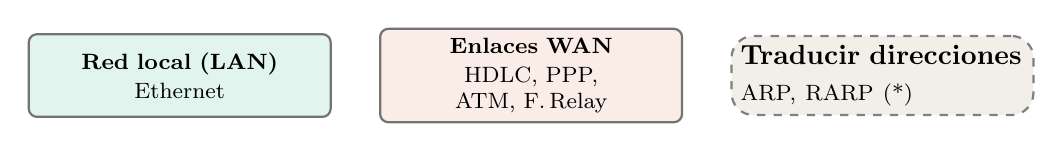
\begin{tikzpicture}[node distance=6mm]
\node[capa=uniTealBg, text width=3.6cm] (lan) {\textbf{Red local (LAN)}\\[1pt]\footnotesize Ethernet};
\node[capa=uniCoralBg, text width=3.6cm, right=of lan] (wan) {\textbf{Enlaces WAN}\\[1pt]\footnotesize HDLC, PPP, ATM, F.\,Relay};
\node[contenedor, draw=black!50, fill=uniGrayBg, text width=3.6cm, right=of wan] (arp) {\textbf{Traducir direcciones}\\[1pt]\footnotesize ARP, RARP (*)};
\end{tikzpicture}
\caption{(*) ``\textit{They're closely involved to this layer}'': el propio material del curso marca ARP/RARP como un caso especial, no de lleno en esta capa.}
\end{figure}

\textbf{HDLC:} protocolo bit-orientado en enlaces WAN punto a punto (encapsulamiento por defecto en interfaces seriales Cisco). \textbf{PPP:} estándar abierto para enlaces punto a punto (dial-up, DSL, algunas VPN), con autenticación integrada (PAP/CHAP) que HDLC no ofrece de forma estándar. \textbf{ATM:} usa celdas de tamaño \emph{fijo} de 53 bytes (5 encabezado + 48 datos), pensado para tráfico predecible tipo voz/video. \textbf{Frame Relay:} tecnología WAN más simple que su predecesor X.25, hoy reemplazada en gran parte por MPLS.

\begin{examfact}
Esta es la única capa con \textbf{dos} etiquetas de encapsulamiento en el diagrama: \textbf{H2} (encabezado) y \textbf{T2} (cola/\textit{trailer}, el FCS). Después de esta capa ya no hay estructura: la capa Física solo transmite bits (\texttt{10101000000010}), sin PDU con encabezado propio.
\end{examfact}

\newpage
% ============================================================
\section{Capa 1 --- Física}
% ============================================================
\textit{Responsable de proveer las especificaciones mecánicas y eléctricas.} PDU: \textbf{Bit} (sin encabezado propio).

La capa Física es la única que no agrega ningún encabezado: solo transmite los bits tal cual, como pulsos eléctricos, luz o señales de radio, a través del ``medio de transmisión''.

\textbf{Interfaces seriales para WAN:} EIA/TIA-449, EIA-530, V.35, RS232, HSSI --- especificaciones mecánicas y eléctricas para conectar un router a un enlace WAN de alta velocidad (vía CSU/DSU). RS232 sigue vivo hoy como el puerto de consola de routers/switches. HSSI fue diseñado por Cisco para enlaces de muy alta velocidad (hasta 52~Mbps, líneas T3).

\textbf{Medios físicos de LAN:} 100BASE-TX y fibra óptica. Ethernet abarca dos capas: su formato de trama es capa 2, pero sus variantes de velocidad y medio son especificaciones de capa 1.

% ---------------- DIAGRAMA 12: decodificar 100BASE-TX ----------------
\begin{figure}[h]
\centering
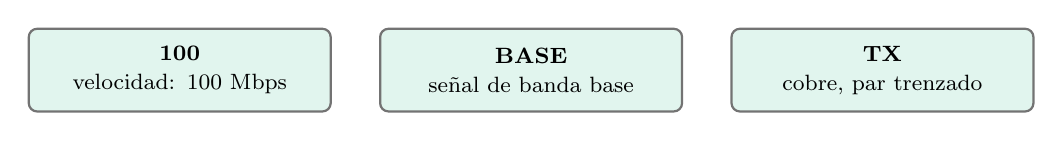
\begin{tikzpicture}[node distance=6mm]
\node[capa=uniTealBg, text width=3.6cm] (n1) {\textbf{100}\\[1pt]\footnotesize velocidad: 100 Mbps};
\node[capa=uniTealBg, text width=3.6cm, right=of n1] (n2) {\textbf{BASE}\\[1pt]\footnotesize señal de banda base};
\node[capa=uniTealBg, text width=3.6cm, right=of n2] (n3) {\textbf{TX}\\[1pt]\footnotesize cobre, par trenzado};
\end{tikzpicture}
\caption{Cómo leer el nombre de un estándar Ethernet: [Velocidad][BASE][Medio].}
\end{figure}

Con ese patrón: \textbf{10BASE-T} = 10~Mbps sobre par trenzado; \textbf{1000BASE-T} = 1~Gbps sobre par trenzado; \textbf{100BASE-FX} = 100~Mbps sobre fibra óptica (F de \textit{fiber}).

\begin{examfact}
Si preguntan ``¿en qué capa está Ethernet?'', la respuesta correcta suele ser ``depende de qué aspecto: su trama es capa 2, sus variantes de velocidad/medio son capa 1''.
\end{examfact}

\newpage
% ============================================================
\section{Tabla maestra: las 7 capas, PDU, función y ejemplos}
% ============================================================

% ---------------- DIAGRAMA 13: host layers vs media layers ----------------
\begin{figure}[h]
\centering
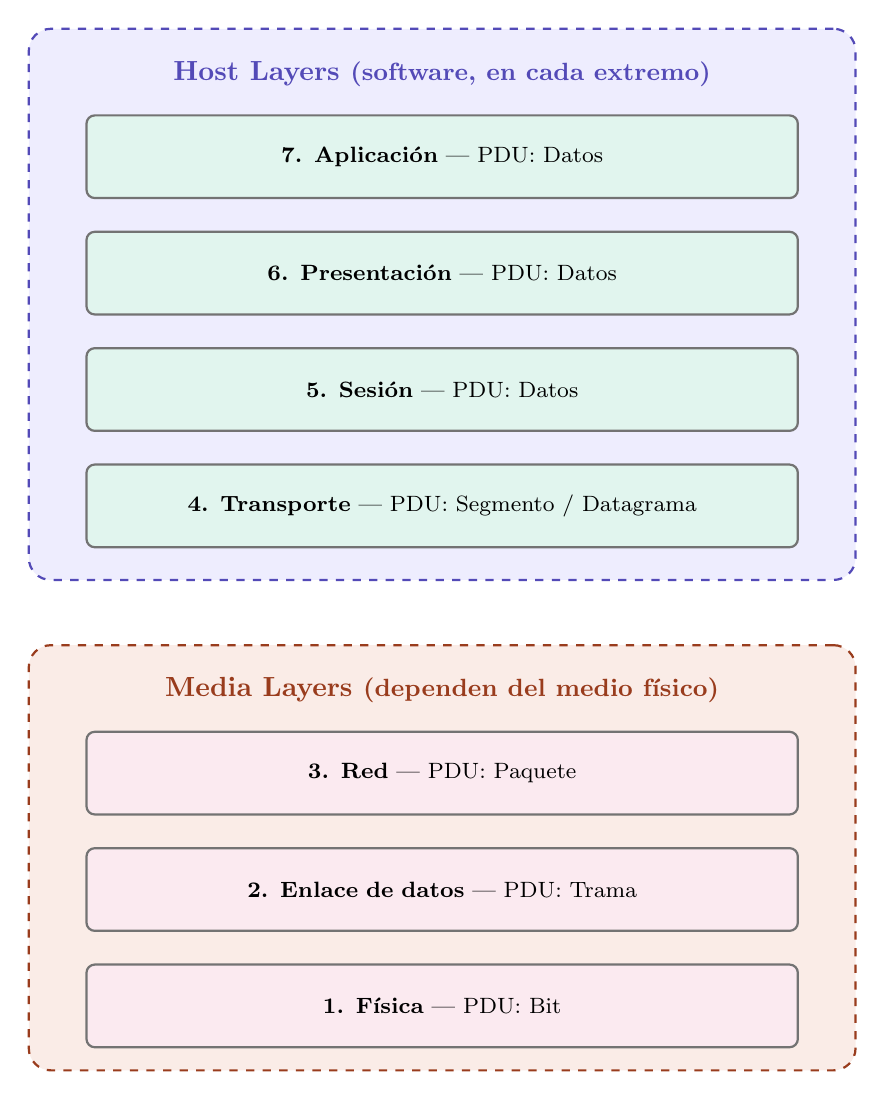
\begin{tikzpicture}[node distance=3mm]
\node[contenedor, draw=uniPurple, fill=uniPurpleBg, minimum width=10.5cm, minimum height=7.0cm] (host) {};
\node[anchor=north, yshift=-3mm, font=\bfseries\color{uniPurple}] at (host.north) {Host Layers \small(software, en cada extremo)};

\node[capa=uniTealBg, text width=8.8cm, below=1.1cm of host.north] (h7) {\textbf{7. Aplicación} --- PDU: Datos};
\node[capa=uniTealBg, text width=8.8cm, below=4mm of h7] (h6) {\textbf{6. Presentación} --- PDU: Datos};
\node[capa=uniTealBg, text width=8.8cm, below=4mm of h6] (h5) {\textbf{5. Sesión} --- PDU: Datos};
\node[capa=uniTealBg, text width=8.8cm, below=4mm of h5] (h4) {\textbf{4. Transporte} --- PDU: Segmento / Datagrama};

\node[contenedor, draw=uniCoral, fill=uniCoralBg, minimum width=10.5cm, minimum height=5.4cm, below=8mm of host] (media) {};
\node[anchor=north, yshift=-3mm, font=\bfseries\color{uniCoral}] at (media.north) {Media Layers \small(dependen del medio físico)};

\node[capa=uniPinkBg, text width=8.8cm, below=1.1cm of media.north] (m3) {\textbf{3. Red} --- PDU: Paquete};
\node[capa=uniPinkBg, text width=8.8cm, below=4mm of m3] (m2) {\textbf{2. Enlace de datos} --- PDU: Trama};
\node[capa=uniPinkBg, text width=8.8cm, below=4mm of m2] (m1) {\textbf{1. Física} --- PDU: Bit};
\end{tikzpicture}
\caption{Las 4 capas de arriba son puro software (Host Layers); las 3 de abajo dependen del medio físico (Media Layers). Transporte es la frontera --- por eso se le llama ``el corazón del OSI''.}
\end{figure}

\begin{examfact}
Esta misma frontera (Host vs.\ Media) es la razón por la que TCP/IP fusiona 3 capas en una (Aplicación) pero deja Transporte intacto: no es casualidad, sigue la misma lógica de qué es ``puro software'' y qué no.
\end{examfact}

\begin{center}
\small
\begin{tabularx}{\textwidth}{@{}l l X X@{}}
\toprule
\textbf{Capa} & \textbf{PDU} & \textbf{Función} & \textbf{Ejemplos} \\
\midrule
Aplicación & Datos & APIs de alto nivel: compartir recursos, acceso remoto a archivos, servicios de directorio, terminales virtuales & RPC, SCP, NFS, PAP, TLS, FTP, HTTP, HTTPS, SMTP, SSH, DNS, LDAP \\
Presentación & Datos & Traducción entre un servicio de red y una aplicación; codificación de caracteres, compresión, cifrado/descifrado & (incluido arriba) \\
Sesión & Datos & Gestión de sesiones de comunicación: intercambio continuo entre dos nodos & (incluido arriba) \\
Transporte & Segmento (TCP) / Datagrama (UDP) & Transmisión confiable de segmentos entre puntos de la red: segmentación, acuse de recibo, multiplexación & TCP, UDP, RTP, SCTP, DCCP \\
Red & Paquete & Estructura y gestión de una red multi-nodo: direccionamiento, ruteo, control de tráfico & ICMP, IGMP, IPsec, ARP, RARP, IPv4, IPv6 \\
Enlace de datos & Trama & Transmisión confiable de tramas entre dos nodos conectados por una capa física & DSL, DOCSIS, MAC, L2TP, LLDP, PPP, IEEE~802.2 \\
Física & Bit & Transmisión y recepción de flujos de bits crudos sobre un medio físico & DSL, DOCSIS, 100BASE-TX \\
\bottomrule
\end{tabularx}
\end{center}

\subsection*{Protocolos nuevos de esta tabla}
\textbf{RTP} (\textit{Real-time Transport Protocol}): corre sobre UDP, agrega marcas de tiempo y números de secuencia para audio/video en tiempo real. \textbf{SCTP}: confiable como TCP pero con varios \textit{streams} independientes dentro de una misma conexión --- si uno pierde un paquete no bloquea a los demás (señalización telefónica, WebRTC). \textbf{DCCP}: como UDP, pero con control de congestión incorporado. \textbf{IGMP}: gestiona grupos de \textit{multicast} (por ejemplo, IPTV). \textbf{L2TP}: túneles de capa 2 sobre una red IP, muy usado en VPN junto con IPsec. \textbf{LLDP}: permite que switches/routers se ``presenten'' a sus vecinos directos para armar el mapa de topología. \textbf{IEEE~802.2}: define la subcapa LLC de Ethernet.

\begin{examfact}
DSL y DOCSIS aparecen listados tanto en Enlace de datos como en Física --- el mismo fenómeno que Ethernet/100BASE-TX: son tecnologías que definen tanto el formato de trama (capa 2) como la especificación eléctrica de la señal (capa 1).
\end{examfact}

\begin{examfact}
SCTP resuelve un problema real de TCP: si un segmento se pierde, TODO se bloquea hasta retransmitirlo (\textit{head-of-line blocking}); SCTP lo evita con \textit{streams} independientes dentro de la misma conexión.
\end{examfact}

\newpage
% ============================================================
\section{Ejemplo integrador: una videollamada de Skype}
% ============================================================

\begin{analogybox}
Estás en una videollamada de Skype desde tu laptop (Red~A), hablando con alguien que tiene su teléfono en otra red (Red~B) --- y al mismo tiempo le mandas un mensaje de texto y le compartes una foto de un gato. Un solo recorrido de principio a fin por las 7 capas.
\end{analogybox}

\subsection*{Bajando las capas en la laptop (Red A)}
\begin{description}[leftmargin=2.6cm, style=nextline]
\item[Capa 7 --- Aplicación] Skype usa sus propios protocolos de capa de aplicación para pedir y enviar datos. Aquí nace el contenido real: voz, texto, foto.
\item[Capa 6 --- Presentación] El audio, texto e imagen se traducen a binario y se cifran antes de salir de la laptop.
\item[Capa 5 --- Sesión] Decide qué paquetes pertenecen a qué archivo: dentro de una sola sesión activa hay tres flujos simultáneos (audio, texto, foto) y la capa de Sesión evita que se mezclen entre sí.
\item[Capa 4 --- Transporte] Segmenta cada flujo. Probablemente no todos usan el mismo protocolo: el audio en vivo viaja por RTP sobre UDP (prioriza velocidad), mientras texto y foto probablemente van por TCP (prioriza integridad).
\item[Capa 3 --- Red] Aquí aparece el paquete con \textbf{IP1} e \textbf{IP2} (laptop y teléfono). Decide la mejor ruta entre Red~A y Red~B, probablemente a través de varios routers intermedios.
\item[Capa 2 --- Enlace de datos] El paquete se envuelve en una trama con \textbf{MAC1}, \textbf{MAC2} y el \textit{trailer} FCS. La IP se mantiene igual durante todo el viaje; las MAC cambian en cada salto.
\item[Capa 1 --- Física] Todo se convierte en señales: fibra óptica entre routers, Wi-Fi en el último tramo hacia cada dispositivo.
\end{description}

% ---------------- DIAGRAMA 14: profundidad de procesamiento por salto ----------------
\begin{figure}[h]
\centering
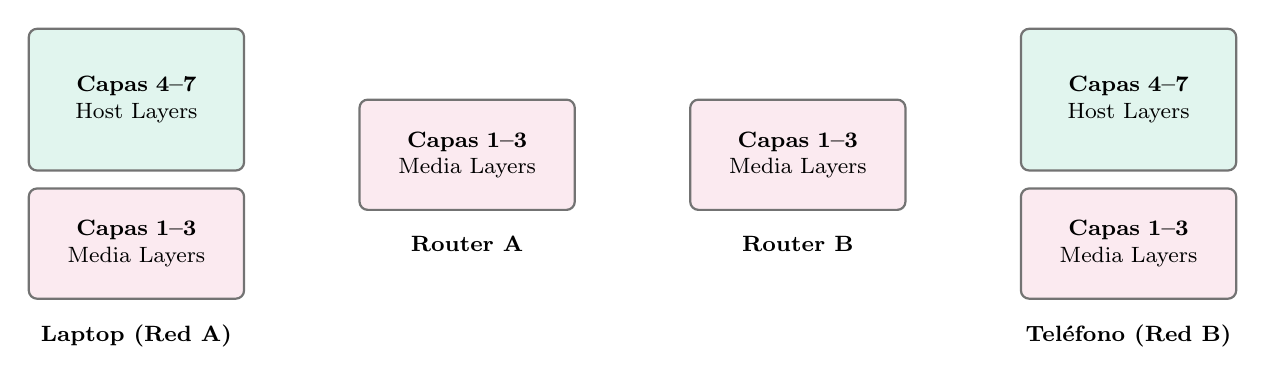
\begin{tikzpicture}[node distance=0mm]
% Laptop
\node[capa=uniTealBg, text width=2.5cm, minimum height=1.8cm] (l47) at (0,2.0) {\footnotesize\textbf{Capas 4--7}\\Host Layers};
\node[capa=uniPinkBg, text width=2.5cm, minimum height=1.4cm, below=2mm of l47] (l13) {\footnotesize\textbf{Capas 1--3}\\Media Layers};
\node[below=2mm of l13, font=\footnotesize\bfseries] {Laptop (Red A)};

% Router A
\node[capa=uniPinkBg, text width=2.5cm, minimum height=1.4cm] (ra) at (4.2,1.3) {\footnotesize\textbf{Capas 1--3}\\Media Layers};
\node[below=2mm of ra, font=\footnotesize\bfseries] {Router A};

% Router B
\node[capa=uniPinkBg, text width=2.5cm, minimum height=1.4cm] (rb) at (8.4,1.3) {\footnotesize\textbf{Capas 1--3}\\Media Layers};
\node[below=2mm of rb, font=\footnotesize\bfseries] {Router B};

% Teléfono
\node[capa=uniTealBg, text width=2.5cm, minimum height=1.8cm] (t47) at (12.6,2.0) {\footnotesize\textbf{Capas 4--7}\\Host Layers};
\node[capa=uniPinkBg, text width=2.5cm, minimum height=1.4cm, below=2mm of t47] (t13) {\footnotesize\textbf{Capas 1--3}\\Media Layers};
\node[below=2mm of t13, font=\footnotesize\bfseries] {Teléfono (Red B)};
\end{tikzpicture}
\caption{Los routers intermedios solo procesan hasta la capa de Red (1--3); solo los dispositivos finales procesan las 7 capas completas.}
\end{figure}

\begin{examfact}
La dirección IP se mantiene igual (origen$\to$destino) durante todo el recorrido; la dirección MAC cambia en cada salto porque solo describe el tramo local entre un dispositivo y el siguiente. De las preguntas más repetidas en examen.
\end{examfact}

\begin{examfact}
Los routers operan hasta la capa 3 (Red); los switches operan en capa 2 (Enlace de datos); solo los dispositivos finales procesan las 7 capas completas.
\end{examfact}

\subsection*{Subiendo las capas en el teléfono (Red B)}
El proceso se invierte exactamente igual: capa Física recibe señales y las convierte en bits, Enlace de datos verifica el FCS y quita las MAC, Red confirma que IP2 es la suya, Transporte reensambla los segmentos de cada flujo por separado, Sesión reordena y separa qué paquetes eran de cada flujo, Presentación descifra y decodifica, y Aplicación (Skype) entrega la llamada, el mensaje y la foto --- correctamente separados y sincronizados, aunque viajaron entremezclados por la misma conexión.

\newpage
% ============================================================
\section{Encapsulamiento completo: cierre del curso}
% ============================================================

% ---------------- DIAGRAMA 15: campos de encapsulamiento ----------------
\begin{figure}[h]
\centering
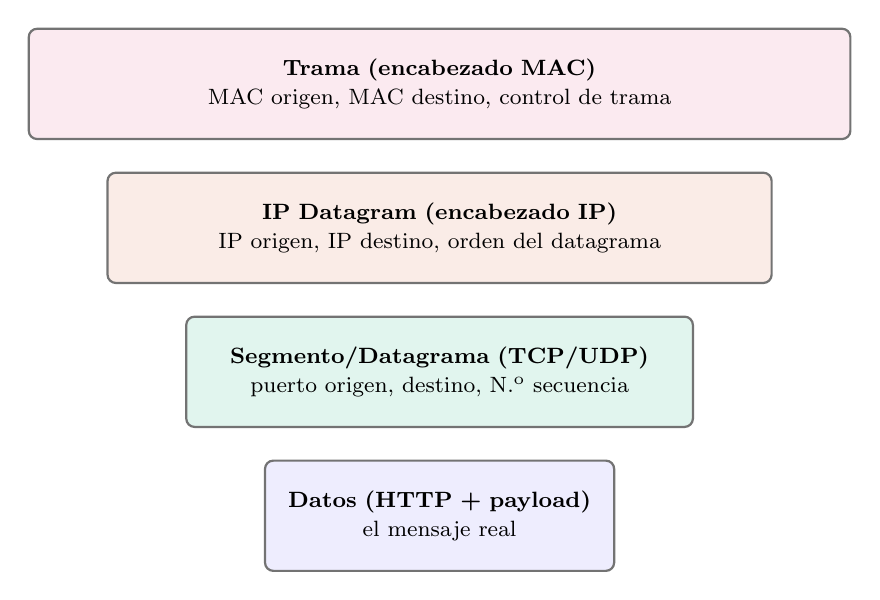
\begin{tikzpicture}[node distance=4mm]
\node[capa=uniPinkBg, text width=10.2cm, minimum height=1.4cm] (fr) {\textbf{Trama (encabezado MAC)}\\[1pt]\footnotesize MAC origen, MAC destino, control de trama};
\node[capa=uniCoralBg, text width=8.2cm, minimum height=1.4cm, below=of fr] (ip) {\textbf{IP Datagram (encabezado IP)}\\[1pt]\footnotesize IP origen, IP destino, orden del datagrama};
\node[capa=uniTealBg, text width=6.2cm, minimum height=1.4cm, below=of ip] (tcp) {\textbf{Segmento/Datagrama (TCP/UDP)}\\[1pt]\footnotesize puerto origen, destino, N.\textsuperscript{o} secuencia};
\node[capa=uniPurpleBg, text width=4.2cm, minimum height=1.4cm, below=of tcp] (data) {\textbf{Datos (HTTP + payload)}\\[1pt]\footnotesize el mensaje real};
\end{tikzpicture}
\caption{Campos concretos dentro de cada encabezado, de afuera hacia adentro.}
\end{figure}

\begin{examfact}
``IP Datagram'' y ``Paquete'' son el mismo concepto: el primero es el término técnico correcto (IP es no orientado a conexión, como UDP), el segundo el más usado coloquialmente.
\end{examfact}

Los campos de ``orden del datagrama'' en el encabezado IP son los de fragmentación (identificación y desplazamiento de fragmento) --- los mismos que permiten el reensamblaje visto en la capa de Red. Los campos ``\textit{frame control}'' y ``\textit{sequence control}'' del encabezado MAC no son para direccionamiento: controlan el tipo de trama y ayudan a detectar tramas duplicadas o fuera de orden (muy usado en Wi-Fi).

\subsection*{Tabla resumen final (en español)}
\begin{center}
\small
\begin{tabularx}{\textwidth}{@{}l l X X@{}}
\toprule
\textbf{Capa} & \textbf{Denominación} & \textbf{Descripción / función} & \textbf{Protocolos conocidos} \\
\midrule
7 & Aplicación & Interactúa con la aplicación informática; ``consume'' lo enviado por el otro extremo & HTTP, FTP, SMTP \\
6 & Presentación & Traducción de datos entre el formato de la aplicación y un formato común; descifrado/cifrado & Esquemas XML, SSL, JPG, MP3/4, DOCX, XLS \\
5 & Sesión & Establece, gestiona y termina sesiones de comunicación entre aplicaciones & NetBIOS, UDP \\
4 & Transporte & Entrega confiable de datos de un extremo a otro; paso de A a B & TCP/IP, UDP \\
3 & Red & Enrutamiento (camino) de paquetes de datos entre redes diferentes & TCP/IP, UDP \\
2 & Enlace & Gestiona el acceso al medio físico; detecta y corrige errores de nivel físico & USB, RJ45, Bluetooth, WiFi, MAC, CSMA/CD \\
1 & Físico & Transmisión y recepción de bits a través de un medio físico: cables, fibra óptica, ondas de radio & Dirección IP para red \\
\bottomrule
\end{tabularx}
\end{center}

\begin{examfact}
La capa de Presentación se describe formalmente en términos de \textbf{sintaxis} (cómo está estructurado el dato) y \textbf{semántica} (qué significa). Ambos extremos deben compartir la sintaxis para interpretar la misma semántica, aunque usen software distinto.
\end{examfact}

\begin{examfact}
\textbf{CSMA/CD} es un \emph{método de acceso al medio}, no un protocolo de trama --- no confundirlo con Ethernet, PPP o HDLC. En redes actuales con switches \textit{full-duplex} las colisiones casi no ocurren, así que CSMA/CD casi nunca entra en acción hoy; sigue en los libros porque explica por qué Ethernet se diseñó como se diseñó.
\end{examfact}

\vspace{0.5cm}
\begin{center}
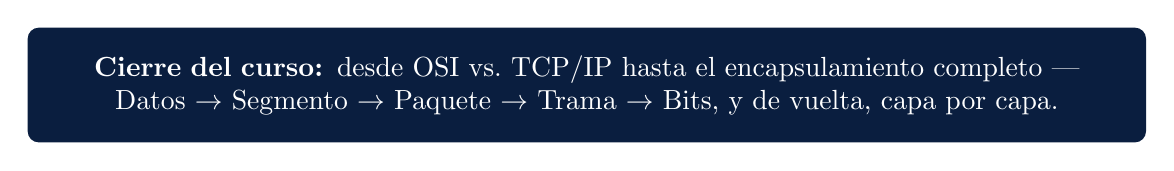
\begin{tikzpicture}
\node[fill=uniDark, text=white, rounded corners=4pt, inner sep=10pt, text width=13.5cm, align=center, font=\normalsize]
  {\textbf{Cierre del curso:} desde OSI vs.\ TCP/IP hasta el encapsulamiento completo --- Datos $\to$ Segmento $\to$ Paquete $\to$ Trama $\to$ Bits, y de vuelta, capa por capa.};
\end{tikzpicture}
\end{center}

\newpage
% ============================================================
\section*{Notas propias}
% ============================================================
\vspace{2cm}
\noindent
\begin{center}
\begin{tikzpicture}
\foreach \i in {0,...,7} {
  \draw[black!40] (0,-\i*1.6) -- (14.2,-\i*1.6);
}
\end{tikzpicture}
\end{center}

\end{document}
